\section{Results}\label{sec:results}

\subsection{The composition mask and what the aggregate cannot identify}\label{sec:mask}

The per-hectare value of capital land $\Ups(q)$ is a concave quadratic in $q$ with an interior maximum at $q^*=q_{\max}/2$, where $\Ups(q^*)=b_c+b_{G,c}\rho_c q_{\max}/4=0.066$ at the baseline; the regenerative term there ($0.016$) is about one third of the direct yield ($0.05$; ratio $0.32$), so capital value is only modestly enhanced by regeneration. The quantity that governs what conversion does to the aggregate is the \emph{composition diagnostic}
\begin{equation}\label{eq:dconv}
\dconv(q,D)=b_f(D)-\Ups(q),
\end{equation}
the difference between what a hectare yields in the fast book and what it is worth in the capital book. At the baseline $\dconv=+0.787,\ +0.784,\ +0.794$ at $q=0.3,\,0.6,\,0.9$: the model sits robustly in the composition-premium regime, in which converting a hectare raises current accounting capacity. The three regimes $\dconv>0$ (premium: conversion raises $B$, mask possible), $\dconv=0$ (first-order neutrality, non-generic) and $\dconv<0$ (discount: conversion lowers $B$ at once, no mask) are the only shape distinction the quality-based model admits; because $Y_c$ is linear in $A_c$ at fixed $q$, there is no area-based capacity maximum and no regime split of the kind an area-based regeneration law would produce.

\begin{proposition}[Composition identity, mask and non-identifiability]\label{prop:mask}
Let $T_b\equiv0$, $R_{rc}\equiv0$ and hold $D$ fixed, so that $b_f$ is constant. Along any solution of \eqref{eq:B}--\eqref{eq:q},
\begin{equation}\label{eq:identity}
\dot B=\dconv(q)\,u_c+b_f\big(\mu A_r-\eta_f A_f\big)+b_{G,c}\,G_c'(q)\,A_c\,\dot q .
\end{equation}
\begin{enumerate}[label=(\roman*)]
\item On any interval on which $u_c>0$, $\dot A_c<0$, and the conversion contribution to $\dot B$ is positive if and only if $\dconv(q)>0$. In the pure-conversion subsystem ($\mu A_r=\eta_f A_f$, $q=q_{\max}$), $\dot B>0\iff\dconv>0$ whenever $u_c>0$: the aggregate rises while the capital book falls.
\item Under frozen demand $E$ and $\dconv>0$, the shortfall $S$ is strictly decreasing along pure conversion ($\dot S=-\dot B<0$ on $S>0$), so the mask is a transient: the trajectory converges to a state with $S=0$ (the balance point of Proposition~\ref{prop:ceiling}) or with $A_c=\Acmin$.
\item The aggregate \eqref{eq:B} is one linear functional of the two areas. From the series $B(t)$ alone, any observed change $\Delta B\ge0$ is consistent with every capital change $\Delta A_c\in[\Acmin-A_c(0),\,0]$ (the fast-book change $\Delta A_f=(\Delta B-\Ups\Delta A_c)/b_f$ absorbs the difference); the capital loss is unidentified. If $b_f$ and $A_f$ are observed independently, the residual $C=B-b_fA_f=\Ups(q)A_c$ identifies the product $\Ups(q)A_c$, but $b_c$, $b_{G,c}$, $\rho_c$ and $q$ enter only through $\Ups=b_c+b_{G,c}\rho_c q(1-q/q_{\max})$ and are not separately identifiable from $C$; the identifiable combinations are $\Ups$ (equivalently $b_{c,\mathrm{eff}}$) and $b_{G,c}\rho_c$.
\end{enumerate}
\end{proposition}

\begin{proof}
Differentiate \eqref{eq:B} with $b_f$ constant and substitute \eqref{eq:Ac}--\eqref{eq:Af} with $R_{rc}=0$: $\dot B=b_f(u_c+\mu A_r-\eta_fA_f)-\Ups u_c+b_{G,c}G_c'(q)A_c\dot q$, which is \eqref{eq:identity}. (i) is immediate from \eqref{eq:identity} and $\dot A_c=-u_c$. (ii) With $\sigma_f=\sigma_c=1$ and $S>0$, $S=E-B$, so $\dot S=-\dot B=-\dconv u_c<0$; $S$ is bounded below by zero and $A_c$ is non-increasing and bounded below by $\Acmin$, so the trajectory converges to a state with $S=0$ or $A_c=\Acmin$. (iii) is the statement that a single linear equation in two unknowns has a one-parameter family of solutions, and that $\Ups$ depends on $(b_c,b_{G,c},\rho_c,q)$ only through the stated combination.
\end{proof}

Figure~\ref{fig:model}a shows the mask at the baseline under frozen demand $E=0.825$ (restoration off, $A_{f0}=0.6$, $A_{c0}=1.5$, $q_0=0.9$, $A_r(0)=0.4$). Biocapacity rises from $0.594$ to $0.825$ ($+39\%$) while capital land falls from $1.500$ to $0.808$ ($-46\%$) and fast land rises from $0.600$ to $0.923$; quality rises from $0.9$ to $1.0$, so the capital \emph{quality} is not drawn down even as its \emph{area} is. The area changes are one-to-one ($\Delta A_f+\Delta A_c+\Delta A_r=0$ to machine precision). The dynamics are fast at first and then asymptotic: because the deficit-side land subsystem is affine (Proposition~\ref{prop:ceiling}(ii)), the approach to the balance point is exponential at the slow rate $|\lambda_1|=0.054\,\mathrm{yr}^{-1}$ (e-folding $\approx19$\,yr), so within $25$\,yr $98\%$ of the rise in $B$ and $85\%$ of the fall in $A_c$ have occurred ($B=0.820$, $A_c=0.913$; $97\%$ of the fall by $50$\,yr), while the strict inequalities $\dot B>0$ and $\dot A_c<0$ persist for $\approx150$\,yr at numerical resolution. The slow tail is reserve equilibration: retirement of fast land to the reserve lowers the fast flow, re-opens a small shortfall, and converts a little more capital, until the reserve reaches its equilibrium share $A_r/A_f=\eta_f/\mu$. The window is therefore not a fixed horizon: its scale is set by $\lambda_1$, which depends on $\tconv$, $\mu$, $\eta_f$ and the yield ratio $b_c/b_f$ (SI~\S S2.2), and its amplitude by $\dconv$ and the initial deficit.

Two consequences of Proposition~\ref{prop:mask}(iii) frame the empirical analysis of Section~\ref{sec:empirical}. First, the composition signature ($B$ rises while $A_c$ falls) is contemporaneously observable only in the two-book series; a monitor who sees the aggregate alone cannot distinguish a composition mask from broad growth. Second, independent proxies for the fast book ($A_f$, $b_f$) convert the aggregate into a measured fast book and a residual, which is the most that can be identified without independent ecological valuation of the capital book. We refer to the two readings as the \emph{composition mask} ($B$ rises while $A_c$ falls; requires $\dconv>0$) and the \emph{liquidation mask} ($E$ steady while $A_c$ falls; requires nothing); which of the two holds is itself a discriminating observable.

\begin{figure}[!htbp]
\centering
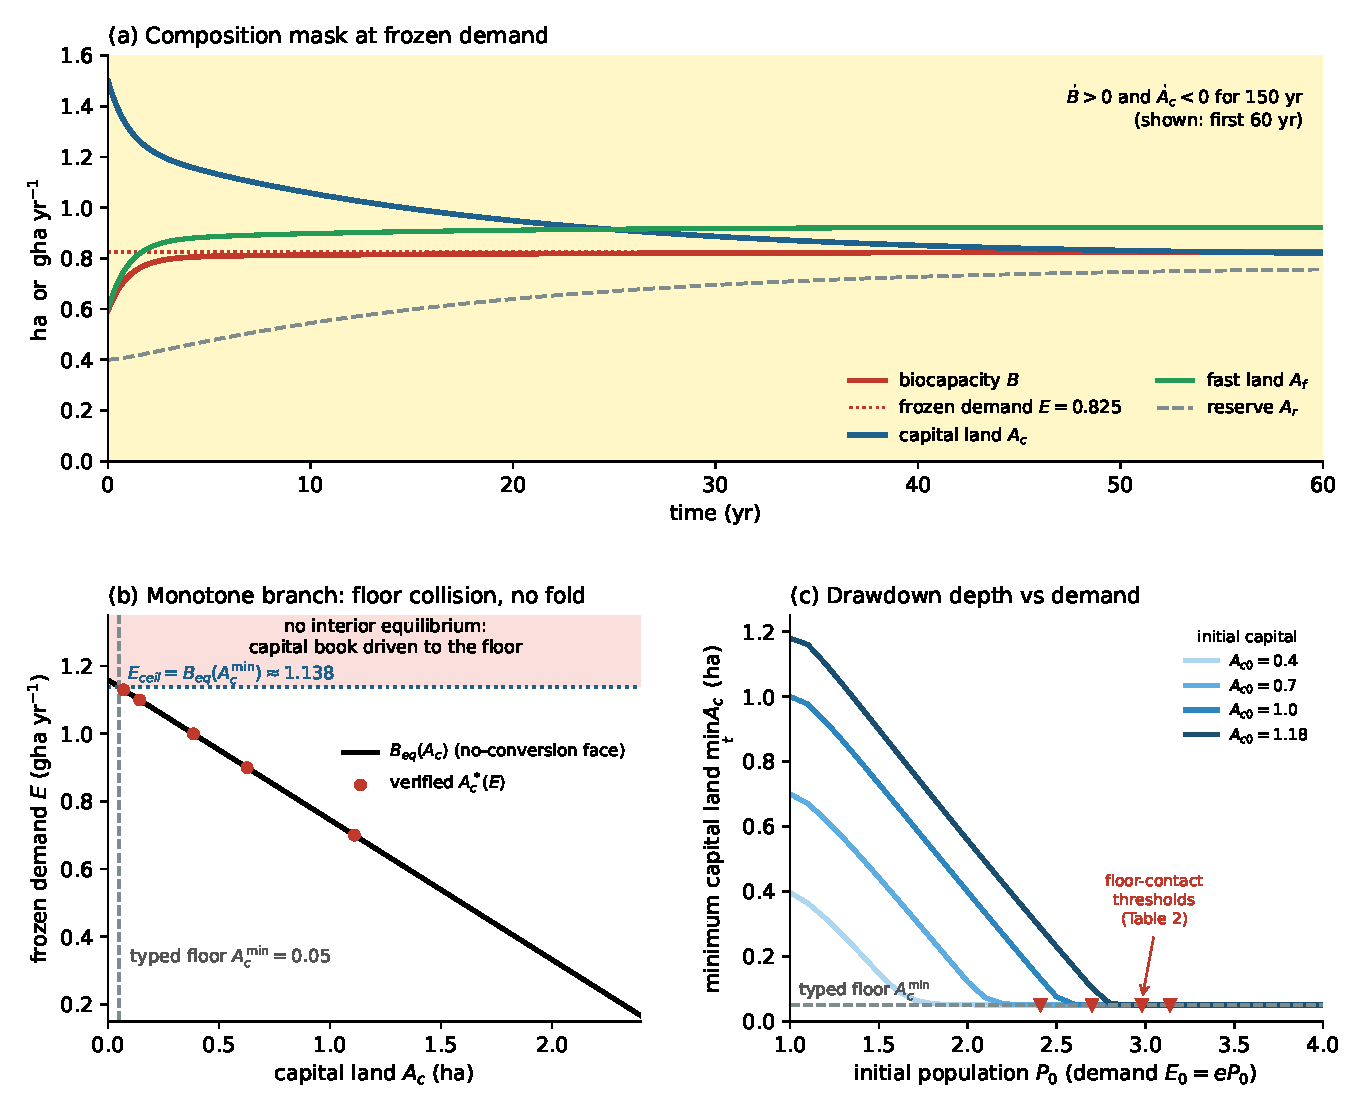
\includegraphics[width=\textwidth]{fig1_model_dynamics}
\caption{Model dynamics at the baseline registry (Table~\ref{tab:params}), regenerated from the deposited code. (a) Composition mask under frozen demand $E=0.825$ (restoration off, $A_{f0}=0.6$, $A_{c0}=1.5$, $q_0=0.9$): biocapacity $B$ rises from $0.594$ to $0.825$ while capital land $A_c$ falls from $1.500$ to $0.808$ and fast land $A_f$ rises from $0.600$ to $0.923$; the shaded region marks the interval on which $\dot B>0$ and $\dot A_c<0$ hold simultaneously ($\approx150$\,yr at numerical resolution; only the first 60\,yr are shown; $98\%$ of the rise in $B$ and $85\%$ of the fall in $A_c$ occur within the first 25\,yr). (b) The frozen-demand balance branch $B_{eq}(A_c)$ of Proposition~\ref{prop:ceiling}, strictly decreasing in $A_c$, with the verified balance points $A_c^*(E)=1.110,\,0.626,\,0.385,\,0.143,\,0.070$ at $E=0.70,\,0.90,\,1.00,\,1.10,\,1.13$; the branch meets the typed floor $\Acmin=0.05$ at the demand ceiling $\Eceil\approx1.138$, above which no balance point exists and the capital book is driven to the floor (shaded). (c) Endogenous-demand runs ($\tau_g=20$, $\tau_p=25$\,yr, $\chi_r=0.10$): the minimum capital land reached during a run is a continuous, monotone function of initial demand $P_0$ (hence $E_0=eP_0$) for each initial capital $A_{c0}$; the floor is approached asymptotically, and the floor-contact thresholds of Table~\ref{tab:model} (triangles) are the operational points at which the floor is reached to within $10^{-6}$. There is no discontinuity in the outcome as a function of demand.}
\label{fig:model}
\end{figure}

\subsection{The drawdown is a demand-driven floor collision, not a fold}\label{sec:ceiling}

With endogenous population there is no interior steady state with active conversion: at a demographic equilibrium $P=K=B/e$, so $E=B$ and $S=0$. Conversion is therefore a transient regime, and its steady states exist only under a frozen exogenous demand pinned above the flow. The frozen-demand system is where the question of a catastrophic shift must be posed, and it has a complete answer.

\begin{proposition}[Balance point, demand ceiling and affine deficit-side dynamics]\label{prop:ceiling}
Assume frozen demand $E$, $T_b\equiv0$, $R_{rc}\equiv0$, $q=q_{\max}$ (the attractor of \eqref{eq:q} for $q(0)>0$) and $D=0$. Let $k=\mu/(\mu+\eta_f)$ and
\begin{equation}\label{eq:Beq}
B_{eq}(A_c)=b_{f0}\,k\,(A_{tot}-A_c)+b_cA_c=b_{f0}kA_{tot}-(b_{f0}k-b_c)A_c .
\end{equation}
\begin{enumerate}[label=(\roman*)]
\item Equilibria of the land subsystem on the no-conversion face $S=0$ satisfy $A_f=k(A_{tot}-A_c)$, $A_r=(1-k)(A_{tot}-A_c)$ and $B_{eq}(A_c)\ge E$. If $b_{f0}k>b_c$, $B_{eq}$ is strictly decreasing, so the balance point $B_{eq}(A_c^*)=E$ is unique,
\begin{equation}\label{eq:Acstar}
A_c^*(E)=\frac{b_{f0}kA_{tot}-E}{b_{f0}k-b_c},
\end{equation}
and it lies above the typed floor if and only if $E<\Eceil:=B_{eq}(\Acmin)$.
\item On the deficit side ($S>0$, $S/b_f<A_c-\Acmin$) the land subsystem is affine in $z=(A_f,A_c)$, $\dot z=Jz+c$, with
\begin{equation}\label{eq:J}
J=\begin{pmatrix}-\tconv^{-1}-\mu-\eta_f & -\mu-\dfrac{b_c}{b_f\tconv}\\[8pt] \tconv^{-1} & \dfrac{b_c}{b_f\tconv}\end{pmatrix},
\qquad \det J=\frac{\mu+\eta_f}{\tconv}\Big(k-\frac{b_c}{b_f}\Big),
\end{equation}
and $\operatorname{tr}J<0$.
$J$ does not depend on $E$ or on the state, $\det J>0$ exactly when $B_{eq}$ is decreasing, and the fixed point of the affine system is the balance point of (i). For $E<\Eceil$ the balance point is admissible and every trajectory that remains in this regime converges to it at the constant rates given by the eigenvalues of $J$; for $E>\Eceil$ the fixed point lies below the floor, the trajectory reaches the face $A_c=\Acmin$ and remains there with a persistent shortfall $S^*=E-\Eceil>0$. The ceiling is a collision of the equilibrium with a face of the admissible set, not a bifurcation of the vector field: there is no second branch, no fold, no hysteresis, and the leading eigenvalue does not tend to zero as $E\to\Eceil$.
\item Beyond the ceiling, with degradation active, the debt converges to the unique root $D^*(E)$ of $\eta D=E-B_{eq}(\Acmin;D)$, where $B_{eq}(\cdot\,;D)$ uses $b_{f0}e^{-\alpha D}$, provided $\eta>\alpha b_{f0}k(A_{tot}-\Acmin)$; $D^*$ is increasing in $E$.
\end{enumerate}
\end{proposition}

\begin{proof}
(i) With $S=0$ and $R_{rc}=0$, \eqref{eq:Af} gives $\mu A_r=\eta_fA_f$, hence $A_r/A_f=\eta_f/\mu$ and, with $A_r=A_{tot}-A_f-A_c$, $A_f=k(A_{tot}-A_c)$; substituting into \eqref{eq:B} with $q=q_{\max}$ ($\Ups=b_c$) and $D=0$ gives $B=B_{eq}(A_c)$, and $S=0$ requires $B\ge E$. Strict monotonicity and \eqref{eq:Acstar} follow from $b_{f0}k>b_c$. (ii) On the deficit side $u_c=(E-b_fA_f-b_cA_c)/(b_f\tconv)$ is affine in $z$; substituting into \eqref{eq:Ac}--\eqref{eq:Af} with $A_r=A_{tot}-A_f-A_c$ gives $J$ and a constant vector $c$ by direct differentiation; $\det J$ follows by expansion, and $\operatorname{tr}J=-\tconv^{-1}(1-b_c/b_f)-\mu-\eta_f<0$ for $b_c<b_f$. The fixed point solves $u_c=0$ and $\mu A_r=\eta_fA_f$, i.e.\ it is the balance point. Because $J$ is constant, convergence rates are constant along the branch. (iii) The map $D\mapsto\eta D+B_{eq}(\Acmin;D)-E$ is continuous, negative at $D=0$ when $E>\Eceil$, tends to $+\infty$, and is strictly increasing when $\eta>\alpha b_{f0}k(A_{tot}-\Acmin)\ge-\partial_DB_{eq}$; hence it has a unique root, which increases with $E$.
\end{proof}

At the baseline $k=0.5455$, the slope $b_{f0}k-b_c=0.414$, and $\Eceil=1.138$; the balance points $A_c^*(E)=1.110,\,0.626,\,0.385,\,0.143,\,0.070$ at $E=0.70,\,0.90,\,1.00,\,1.10,\,1.13$ agree with the integrated equilibria (Fig.~\ref{fig:model}b). The eigenvalues of $J$ are real and negative, $\lambda_1=-0.0537$ and $\lambda_2=-0.998\,\mathrm{yr}^{-1}$; $\lambda_1$ varies only weakly with the fast-land yield, from $-0.0522$ at $b_f=0.60$ to $-0.0556$ at $b_f=2.00$ (Table~\ref{tab:model}a), and never changes sign. There is no universal scalar stability index: the conversion-loop gain is the state- and parameter-dependent $\dconv$, of order $1\,\mathrm{gha\,ha^{-1}\,yr^{-1}}$, and the return rate is $|\lambda_1|$ of order $10^{-2}\,\mathrm{yr}^{-1}$. Beyond the ceiling the debt fixed points are $D^*=1.19$ and $5.38$ at $E=1.158$ and $1.238$ (integrated values $1.21$ and $5.39$); the monotonicity condition of (iii) holds with margin ($\alpha b_{f0}k(A_{tot}-\Acmin)=0.034<\eta=0.05$), so under frozen demand the debt saturates rather than running away.

The statement ``no critical slowing down'' is precise here. By critical slowing down we mean that the least-negative eigenvalue of the relevant linearisation tends to $0^-$ as a parameter approaches a fold, so that the return time $T_{ret}\approx-1/\lambda_1$ diverges. In Proposition~\ref{prop:ceiling} the linearisation is constant along the entire branch, so neither $\lambda_1$ nor $T_{ret}\approx19$\,yr changes as $E\to\Eceil$. The only early-warning signal the model offers is a \emph{boundary} signal, the capital book approaching its typed floor, which is observable only in the two-book series.

With endogenous demand the same structure appears as a continuous drawdown. Figure~\ref{fig:model}c shows the minimum capital land reached during a run as a function of initial population $P_0$ for four initial capital stocks: the curves are continuous and monotone, the floor is approached asymptotically (because $u_c\le(A_c-\Acmin)/\tconv$, the distance to the floor decays exponentially during a sustained deficit and is never crossed), and higher initial capital supports higher demand before the floor is reached. The ``collapse thresholds'' of the earlier literature on this model are therefore operational quantities: Table~\ref{tab:model}b reports the initial demand at which the floor is approached to within $10^{-2}$, $10^{-4}$ and $10^{-6}$ of its value. The $10^{-6}$ floor-contact values ($P_0\approx2.41,\,2.70,\,2.98,\,3.14$ for $A_{c0}=0.40,\,0.70,\,1.00,\,1.18$) are the ones a bisection on exact floor contact returns; they rise monotonically with initial capital, as do the looser criteria, and no criterion exhibits a jump. Two robustness checks bear on the predictions of Section~\ref{sec:predictions}: the floor-contact threshold at $A_{c0}=1.0$ is identical to three decimals for $\tau_g=5$, $20$ and $40$\,yr, and identical to three decimals with the restoration coefficient $\chi_r=0.10$ and $\chi_r=0$ (SI~\S S4). The first reflects the small leverage of the regenerative term at the baseline and the monotone quality dynamics; the second reflects the fact that a surplus-gated flow is inert during the shortfall that produces the drawdown.

\begin{table}[!htbp]
\centering\small
\caption{Model results at the baseline registry. (a) Composition diagnostic at $q^*=q_{\max}/2$ ($\Ups(q^*)=0.066$), eigenvalues of the deficit-side matrix $J$ of \eqref{eq:J} and the demand ceiling, for a sweep of the fast-land yield $b_f$ (all other parameters at baseline). (b) Initial demand $P_0$ (initial footprint $E_0=0.55P_0$) at which the minimum capital land reached during an endogenous-demand run ($A_{f0}=0.6$, $q_0=0.9$, $\tau_g=20$, $\tau_p=25$\,yr) comes within the stated distance of the typed floor $\Acmin=0.05$; the first two columns are read from a $P_0$ grid of step $0.1$ ($\Delta t=0.1$\,yr, $T=400$\,yr), the last is a bisection on exact floor contact ($\Delta t=0.05$\,yr, $T=1000$\,yr). Drawdown depth is continuous in $P_0$ (Fig.~\ref{fig:model}c); the thresholds are a band, not a single value.}
\label{tab:model}
\begin{tabular}{l l l l l}
\toprule
\multicolumn{5}{l}{(a) Fast-land yield sweep (all rows composition-premium, $\dconv>0$)}\\
$b_f$ & $\dconv(q^*)$ & $\lambda_1$ (yr$^{-1}$) & $\lambda_2$ (yr$^{-1}$) & $\Eceil$ \\
\midrule
$0.60$ & $+0.534$ & $-0.0522$ & $-0.975$ & $0.804$ \\
$0.85$ (baseline) & $+0.784$ & $-0.0537$ & $-0.998$ & $1.138$ \\
$1.20$ & $+1.134$ & $-0.0547$ & $-1.014$ & $1.606$ \\
$2.00$ & $+1.934$ & $-0.0556$ & $-1.029$ & $2.675$ \\
\bottomrule
\end{tabular}

\medskip
\begin{tabular}{l l l l}
\toprule
\multicolumn{4}{l}{(b) Initial demand $P_0$ at which $\min_tA_c$ approaches $\Acmin$ to within:}\\
$A_{c0}$ (ha) & within $10^{-2}$ & within $10^{-4}$ & floor contact ($10^{-6}$) \\
\midrule
$0.40$ & $\approx1.8$ & $\approx2.1$ & $\approx2.41$ \\
$0.70$ & $\approx2.2$ & $\approx2.4$ & $\approx2.70$ \\
$1.00$ & $\approx2.6$ & $\approx2.8$ & $\approx2.98$ \\
$1.18$ & $\approx2.8$ & $\approx3.0$ & $\approx3.14$ \\
\bottomrule
\end{tabular}
\end{table}

\subsection{The mask is bounded: technology saturates, debt does not}\label{sec:bounded}

Both the technology wave and the degradation act on the same coefficient, the fast-land yield $b_f$ of \eqref{eq:bf}, and they do so multiplicatively. This yields a structural asymmetry.

\begin{proposition}[Boundedness asymmetry]\label{prop:bounded}
Under \eqref{eq:bf}--\eqref{eq:Tb}:
\begin{enumerate}[label=(\roman*)]
\item the technology factor satisfies $1\le(b_{f0}+T_b(t))/b_{f0}\le1+\Delta b/b_{f0}$ for all $t$, so the logarithmic gain of the yield channel is bounded by $\ln(1+\Delta b/b_{f0})$ uniformly in time ($0.78$ at the baseline);
\item the debt satisfies $D(t)\le\max\{D(0),\ \sup_{s\le t}\pos{E-B}(s)/\eta\}$, and $D\to S^*/\eta$ whenever the shortfall settles at $S^*$; the degradation factor $e^{-\alpha D}$ is therefore bounded below only through the sustained shortfall;
\item the degradation loss exceeds the maximal technology gain once the sustained shortfall exceeds $S^\dagger=(\eta/\alpha)\ln(1+\Delta b/b_{f0})$, equal to $1.30\,\mathrm{gha\,yr^{-1}}$ at the baseline.
\end{enumerate}
Under an additive degradation law $b_f=b_{f0}+T_b-\alpha D$ the two channels enter symmetrically and (iii) reduces to a comparison of $\Delta b$ with $\alpha D^*$; the asymmetry is a property of the multiplicative form.
\end{proposition}

\begin{proof}
(i) is $0\le T_b\le\Delta b$. (ii) From \eqref{eq:D}, $\dot D\le\bar S-\eta D$ with $\bar S=\sup_{s\le t}\pos{E-B}$, so $D(t)\le\max\{D(0),\bar S/\eta\}$ by comparison; if $\pos{E-B}\to S^*$ then $D\to S^*/\eta$. (iii) compares $\alpha S^*/\eta$ with $\ln(1+\Delta b/b_{f0})$.
\end{proof}

The proposition corrects a tempting overstatement: debt does not compound without bound under a fixed shortfall -- it saturates at $S^*/\eta$ -- but its ceiling is set by the shortfall rather than by a parameter, and the shortfall is itself raised by demand growth. At the baseline the crossover shortfall $S^\dagger\approx1.3\,\mathrm{gha\,yr^{-1}}$ exceeds the baseline biocapacity, so at these parameters the debt channel is a slow erosion rather than a reckoning; what bounds the mask at the baseline is the balance-point mechanism of Proposition~\ref{prop:mask}(ii), with debt erosion as the second, slower limit. A second coupling works in the same direction: because $K=B/e$, any technology-driven rise in $B$ raises the carrying capacity and, with the demographic delay, demand; under overshoot the wave that lifts the aggregate also raises the shortfall that feeds $D$ -- a Jevons-type rebound in which technology increases cumulative debt. The mask therefore opens only while the yield gain outpaces the debt build-up, and it is a transient diagnostic, not a new equilibrium.

\subsection{Recovery requires an explicit, gated restoration flow}\label{sec:recovery}

The model is structurally asymmetric: $A_c\to A_f$ proceeds through conversion, but no term in \eqref{eq:Ac}--\eqref{eq:Ar} returns land to the capital book except the restoration flow $R_{rc}$. Fast-land retirement sends land to the reserve, not to capital. Reducing population, footprint or shortfall therefore does not reverse prior conversion: with $\chi_r=0$ the capital book stays where the shortfall left it. In the endogenous-demand run with $A_{c0}=1.0$ and $P_0=2.0$, capital land falls to $0.398$\,ha within four years and remains there without restoration, whereas with the surplus-gated flow ($\chi_r=0.10$) it recovers to $0.828$\,ha, a recovery fraction $\mathcal R_c=(A_c(T)-A_c^{\mathrm{deg}})/(A_c^{\mathrm{init}}-A_c^{\mathrm{deg}})=0.71$ (SI~\S S4.3). The sign of the gate matters. A surplus-gated flow, active when $B>E$, is the ecologically sign-correct rewilding: it retires land only when the system has spare capacity, but it is inert during the shortfall it must eventually address -- which is why the drawdown thresholds of Table~\ref{tab:model}b do not depend on $\chi_r$ -- and once a surplus opens it can over-restore while the supported population re-equilibrates downward, so a target-level stopping rule is needed for a clean $\mathcal R_c=1$ (SI~\S S4.4). A deficit-gated flow, active when $E>B$, is the one gate that acts during the shortfall, but it retires productive land exactly when provision is short and can deepen the near-term deficit; at the tested rates conversion outpaces it, so it is necessary but insufficient and must be sized or capped. Neither gate is an unqualified good, and the gate-sign asymmetry is phase-dependent rather than a universal ranking.

\subsection{Measured composition of aggregate biocapacity, 1961--2022}\label{sec:empirical}

The identity $d\ln B=d\ln(B/P)+d\ln P$ applied to the NFA world series gives the aggregation face of the result (Fig.~\ref{fig:aggregation}). Aggregate biocapacity rose $+23.0\%$ ($\Delta\ln B=+0.207$, $+0.339\%\,\mathrm{yr}^{-1}$); per-capita biocapacity fell $-52.9\%$ ($\Delta\ln(B/P)=-0.752$, $-1.23\%\,\mathrm{yr}^{-1}$); the per-capita footprint rose $+16.9\%$; and the biocapacity ratio $R_B=E/B$ rose from $0.718$ to $1.782$, crossing $1$ in 1971. Because the identity is exact (residual $<10^{-16}$) the split is unambiguous: population contributed $+0.959$ ($+464\%$ of $\Delta\ln B$) and the per-capita term $-0.752$ ($-364\%$). This is the extensive/intensive split, not a causal claim (biocapacity is computed from area and yield independently of $P$), and it is not yet the two-land composition mask: the same aggregate that hides a per-capita halving is the one that would hide a capital-land drawdown.

\begin{figure}[!htbp]
\centering
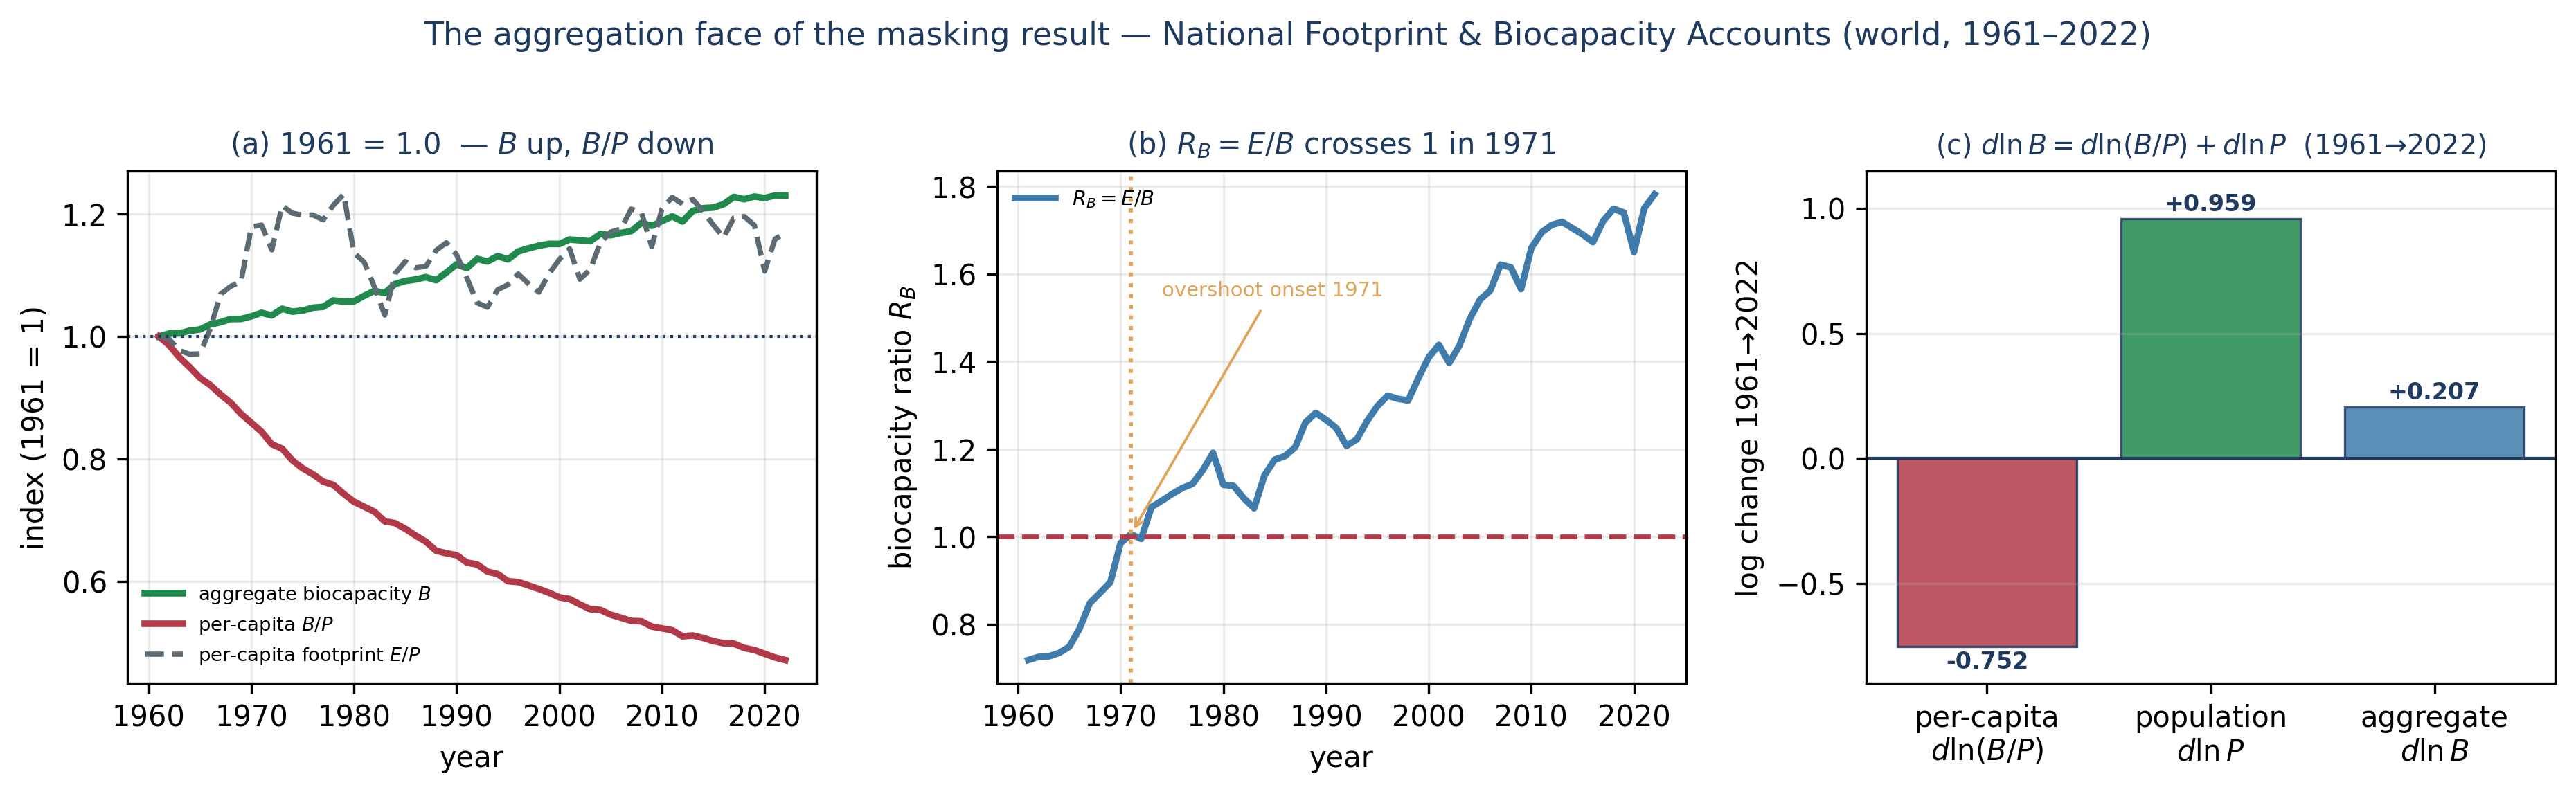
\includegraphics[width=\textwidth]{fig2_nfa_aggregation_face}
\caption{The aggregation face of the masking result, National Footprint and Biocapacity Accounts (world, 1961--2022). (a) Indices (1961 $=1$) of aggregate biocapacity $B$, per-capita biocapacity $B/P$ and per-capita footprint $E/P$: $B$ rises while $B/P$ halves. (b) The biocapacity ratio $R_B=E/B$ crosses $1$ (overshoot onset) in 1971. (c) The exact identity $d\ln B=d\ln(B/P)+d\ln P$: population $+0.959$ and per-capita $-0.752$ (shares of $\Delta\ln B$: $+464\%$ and $-364\%$). The public aggregate carries no yield/area split, so this panel is explicitly not the two-land composition mask.}
\label{fig:aggregation}
\end{figure}

To advance past the aggregate we apply the observation operator of Section~\ref{sec:data}. With $A_f$ from FAOSTAT cropland area and $b_f$ from the normalised crop-yield index calibrated at 1961, the exact Divisia decomposition \eqref{eq:divisia} attributes the $+0.207$ aggregate log-change to a yield channel $+0.393$, a cropland-area channel $+0.056$ and a residual $-0.242$ (Table~\ref{tab:divisia}). Raw component log-changes ($+1.128$, $+0.160$, $-0.404$) are changes in the components, not contributions, and cannot be summed; the log-mean weights $w_X=0.349$, $w_C=0.600$ make the identity exact, whereas average shares ($0.375$, $0.625$) would give $+0.231$. The yield channel dominates the growth of the aggregate, cropland area is a small positive, and the residual -- all biocapacity not captured by the cropland proxy -- is a large negative. The result is robust to the unidentified base-year cropland share: over $\alpha\in[0.10,0.34]$ the weighted identity sums to $+0.207$ exactly and the yield channel is the dominant positive term at every $\alpha$, although the split is not pinned ($w_X$ ranges $0.18$--$0.62$); for $\alpha\ge0.339$ the residual is no longer positive at the endpoint and the level decomposition $\Delta B=\Delta X+\Delta C$ (reproducing $\Delta B=+2.242\times10^{9}$\,gha) carries the same sign statement (SI~\S S5.2). The nominal anchor $\alpha=0.19$ can be replaced by the measured one, $b_f(1961)=B_{\mathrm{cropland,NFA}}(1961)/A_f(1961)\approx0.93\,\mathrm{gha\,ha^{-1}\,yr^{-1}}$ (cropland share $\approx0.128$), which lies inside the robustness band and leaves the decomposition unchanged. The instantaneous fast-book share $s_X$ rises from $0.19$ to $0.56$ over the period; only the growth and sign statements are robust, and $b_c$, $b_{G,c}$, $\rho_c$ and the yield/area split of the residual remain unidentified, exactly as Proposition~\ref{prop:mask}(iii) says they must.

\begin{table}[!htbp]
\centering\small
\caption{Exact log-mean (Divisia) decomposition of world aggregate biocapacity growth, 1961--2022 (NFA aggregate series; cropland proxies from FAOSTAT; base-year calibration $\alpha=0.19$). Contributions sum exactly to $\Delta\ln B=+0.207$. Raw log-changes are component changes, not contributions.}
\label{tab:divisia}
\begin{tabularx}{\textwidth}{X l l l}
\toprule
Component & Raw $\Delta\ln$ & Log-mean weight & Contribution to $\Delta\ln B$ \\
\midrule
Fast-book yield $b_f$ (crop-yield index) & $+1.128$ & $w_X=0.349$ & $+0.393$ \\
Fast-book area $A_f$ (cropland) & $+0.160$ & $w_X=0.349$ & $+0.056$ \\
Residual $C=B-b_fA_f$ (non-cropland) & $-0.404$ & $w_C=0.600$ & $-0.242$ \\
\midrule
Total & & & $+0.207$ \\
\bottomrule
\end{tabularx}
\end{table}

The measured land-type accounts make the composition explicit without any proxy (Fig.~\ref{fig:composition}). In the land-type vintage the aggregate grew $+24.5\%$ ($\Delta\ln B=+0.219$), of which cropland contributed $+23.8$ points and built-up land $+7.3$ points, while forest products, grazing land and fishing grounds together contributed $-6.6$ points; the component ratios are cropland $2.85\times$ (area $1.17\times$, per-hectare yield $2.43\times$), built-up $8.63\times$, forest products $0.90\times$, grazing $0.98\times$, fishing $0.96\times$. Cropland accounts for essentially all of the net aggregate growth ($\approx97$--$103\%$ depending on vintage), and the non-cropland book is flat at the endpoint ($1.008\times$; intra-period index up to $1.024\times$). The identifiability limit is recursive: the near-flat non-cropland total is itself the net of declining forest-products, grazing and fishing biocapacity (together $\approx-6.4\times10^{8}$\,gha) and an $8.6\times$ rise in built-up land. These categories are accounting flows and land classes rather than the model's capital stock, so the accounts do not demonstrate a measured decline in $A_c$; they do demonstrate that aggregate summary statistics conceal composition at more than one level.

\begin{figure}[!htbp]
\centering
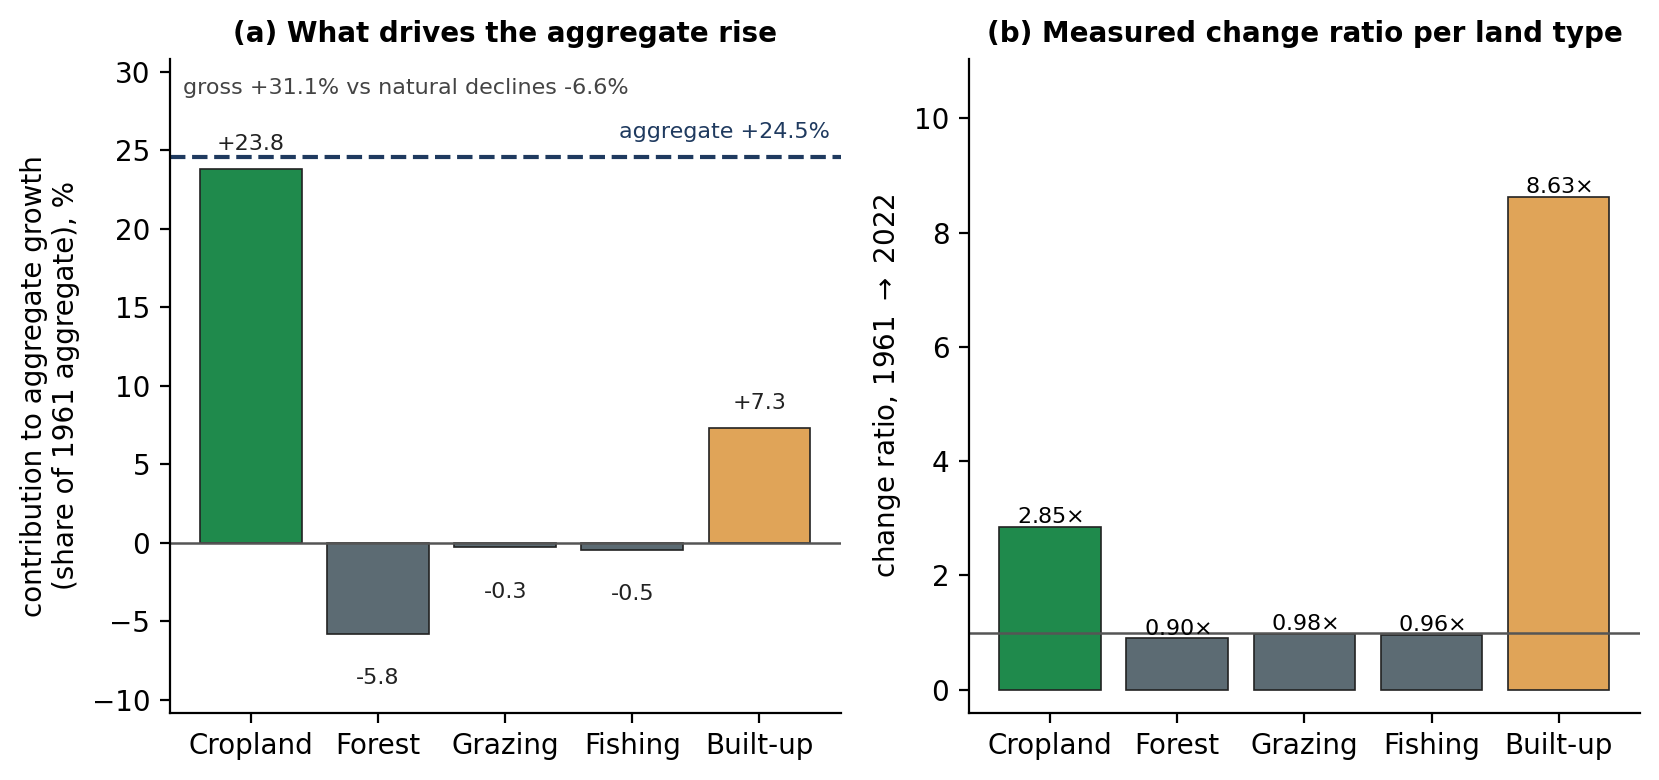
\includegraphics[width=0.95\textwidth]{fig3_composition_attribution}
\caption{Measured land-type composition of aggregate biocapacity change, National Footprint and Biocapacity Accounts (world, 1961--2022, land-type vintage). (a) Contributions to the $+24.5\%$ aggregate growth ($\Delta\ln B=+0.219$): cropland $+23.8$ points and built-up land $+7.3$ points (gross $+31.1$), against forest products, grazing and fishing $-6.6$ points; the components sum exactly to the aggregate. (b) Endpoint ratios: cropland $2.85\times$, built-up $8.63\times$, forest products $0.90\times$, grazing $0.98\times$, fishing $0.96\times$. A single aggregate number cannot reveal this composition.}
\label{fig:composition}
\end{figure}

\subsection{Falsifiable predictions}\label{sec:predictions}

The model's testable content, framed against two-book series ($B$, $A_c$, $A_f$ and land-cover/yield proxies) rather than the aggregate, is the following.
\begin{enumerate}[label=P\arabic*.,leftmargin=2.2em]
\item \textbf{Mask signature.} During conversion $\dot A_c<0$ while $\dot B\ge0$, and $R_B\le1$ is not required: the capital book can fall while the aggregate is at or below demand. Observing $\dot A_c<0$ with a steady or rising $B$ (composition mask) versus a steady $E$ (liquidation mask) discriminates the two readings (Proposition~\ref{prop:mask}).
\item \textbf{Window scale.} The duration of the mask is set by the slow eigenvalue $\lambda_1$ (through $\tconv$, $\mu$, $\eta_f$, $b_c/b_f$) and its amplitude by $\dconv$ and the deficit, not by a fixed horizon; the bulk of conversion precedes the closing of the deficit by one to two e-folding times.
\item \textbf{No critical-slowing precursor.} The return time does not grow as demand approaches the ceiling, and the drawdown depth is continuous in demand (Fig.~\ref{fig:model}c); the observable warning is the capital book approaching its typed floor (Proposition~\ref{prop:ceiling}). This is a negative prediction: a catastrophic-shift early-warning indicator is not expected to precede the two-land drawdown.
\item \textbf{Demand threshold, not delay threshold.} The initial demand that drives the capital book to its floor rises with initial capital (Table~\ref{tab:model}b) and is insensitive to the regeneration delay (identical to $10^{-3}$ for $\tau_g=5$--$40$\,yr), because the regenerative share of capital value is small and quality is monotone; a one-stock regeneration cliff is not expected.
\item \textbf{Recovery requires a gated flow.} Reducing demand does not restore the capital book; recovery requires an explicit restoration flow whose gate sign determines whether it is inert during the shortfall (surplus-gated; thresholds unchanged by $\chi_r$) or deepens it (deficit-gated).
\end{enumerate}
The identifiability statement of Proposition~\ref{prop:mask}(iii) is not a prediction but a constraint on testing: P1--P5 can be tested only with independent $A_c$ and $b_f$ proxies, never with the aggregate alone.

